\documentclass{report}

% Paquetes y configuraciones adicionales
\usepackage{graphicx}
\usepackage[export]{adjustbox}
\usepackage{caption}
\usepackage{float}
\usepackage{titlesec}
\usepackage{geometry}
\usepackage[hidelinks]{hyperref}
\usepackage{titling}
\usepackage{titlesec}
\usepackage{parskip}
\usepackage{wasysym}
\usepackage{tikzsymbols}
\usepackage[english]{babel}

\newcommand{\subtitle}[1]{
  \posttitle{
    \par\end{center}
    \begin{center}\large#1\end{center}
    \vskip0.5em}
}

% Configura los márgenes
\geometry{
    left=2cm,   % Ajusta este valor al margen izquierdo deseado
    right=2cm,  % Ajusta este valor al margen derecho deseado
    top=3cm,
    bottom=3cm,
}

% Configuración de los títulos de las secciones
\titlespacing{\section}{0pt}{\parskip}{\parskip}
\titlespacing{\subsection}{0pt}{\parskip}{\parskip}
\titlespacing{\subsubsection}{0pt}{\parskip}{\parskip}

% Redefinir el formato de los capítulos y añadir un punto después del número
\makeatletter
\renewcommand{\@makechapterhead}[1]{%
  \vspace*{0\p@} % Ajusta este valor para el espaciado deseado antes del título del capítulo
  {\parindent \z@ \raggedright \normalfont
    \ifnum \c@secnumdepth >\m@ne
        \huge\bfseries \thechapter.\ % Añade un punto después del número
    \fi
    \interlinepenalty\@M
    #1\par\nobreak
    \vspace{10pt} % Ajusta este valor para el espacio deseado después del título del capítulo
  }}
\makeatother

% Configura para que cada \chapter no comience en una pagina nueva
\makeatletter
\renewcommand\chapter{\@startsection{chapter}{0}{\z@}%
    {-3.5ex \@plus -1ex \@minus -.2ex}%
    {2.3ex \@plus.2ex}%
    {\normalfont\Large\bfseries}}
\makeatother

\begin{document}

% Portada del informe
\title{IBM Power System AC922}
\subtitle{Arquitecturas Avanzadas y de Propósito Específico}
\author{Carlos Pérez Fino and Cheuk Kelly Ng Pante}
\date{21 of november of 2023}

\maketitle

% Índice
\tableofcontents

% Nueva página para el primer capítulo
\cleardoublepage

\chapter{Introduction}
The IBM Power System AC922 is a powerful computing platform featuring IBM's Power9 processor.
Designed to deliver exceptional performance, this system excels in data-intensive applications and demanding workloads.
data-intensive applications and demanding workloads. With advanced features, the AC922 is a robust choice for
artificial intelligence and big data analytics applications.

% Secciones del informe
% Capitulo 2
\chapter{Multithreading and Multiprocessors}

% 2.1 Multithreading
\section{Multithreading}
The IBM Power System AC922 is a system based on Power9 processor technology, a 64-bit processor that supports simultaneous
multithreading and multiprocessors. The term concurrent multithreading refers to a variation of fine-grained multithreading
that arises naturally when implemented on top of a processor with multiple issue and dynamic scheduling, which is based on
the ability of a system or program to execute multiple threads simultaneously or concurrently. Multithreading is a technique
in programming that allows an application to split its work into smaller tasks and execute them in parallel
tasks and execute them in parallel in multiple threads of execution. This can significantly improve the performance
and responsiveness of an application on systems with multiple processor cores.

When people talk about ``concurrent multithreading'', they are emphasising the idea that multiple threads are running at the same time, making efficient use of hardware resources.

% Poner una imagen
\begin{figure}[H]
  \centering
  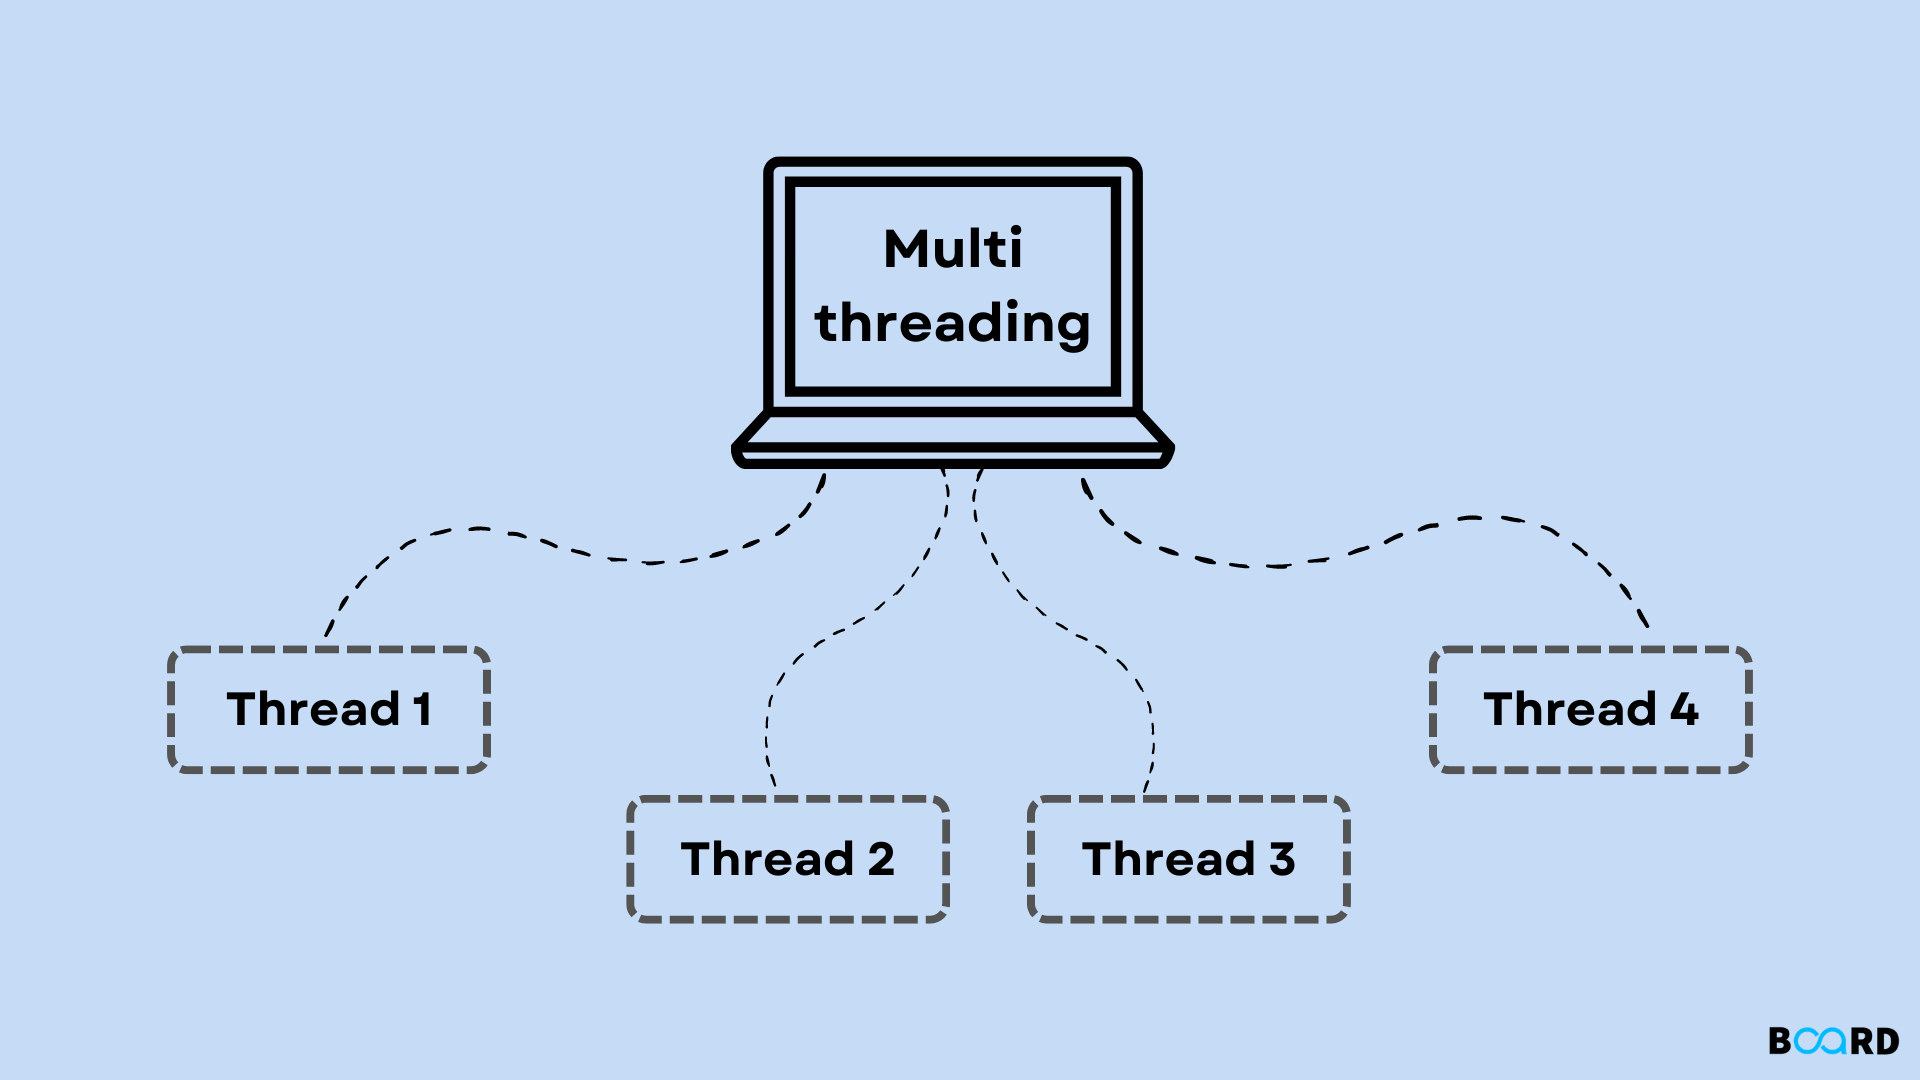
\includegraphics[scale=0.3]{img/multithreading.png}
  \caption{General scheme of multithreading}
  \label{fig:General scheme of multithreading}
\end{figure}

% Nueva página
\cleardoublepage

% 2.2 Multiprocesadores
\section{Multiprocessors}
Power9 also supports multiprocessors, which means that multiple processors can be connected to work together on a task. Multiprocessors 
are computer systems that consist of several processors or processing units working together on a single machine. These processors are
tightly coupled, which means that they are designed to work in close collaboration and coordination with each other. In addition,
they share memory through a shared address space, which allows the processors to access and share data in a common central memory.

\begin{figure}[H]
  \centering
  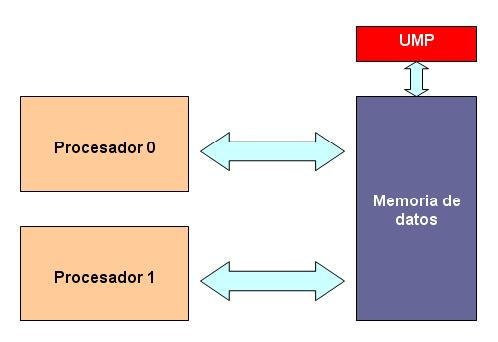
\includegraphics[scale=0.5]{img/multiprocesador.jpg}
  \caption{General scheme of multiprocessor}
  \label{fig:General scheme of multiprocessor}
\end{figure}

There are two major obstacles to be considered in these types of parallel systems. The first has to do with the
the second arises from the relatively high cost of communications (lower between cores and higher when going out to the interconnection network
chip interconnection network). The Power9 processor uses a SMP system (symmetric shared-memory multiprocessors SMP), all the processors have access to the same memory, and all the processors have access to the same memory.
processors have access to the same physical memory, which enables efficient communication between processors and facilitates
processors and facilitates the execution of parallel applications. This architecture is suitable for workloads that
workloads that benefit from fast access to shared memory and the ability to run multiple threads simultaneously.
simultaneously.

\begin{figure}[H]
  \centering
  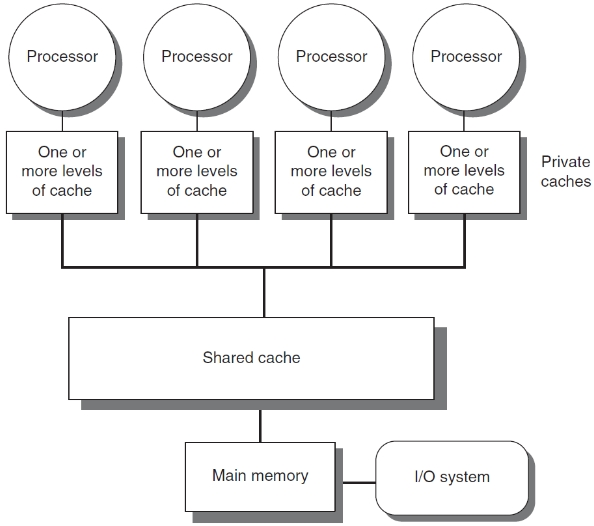
\includegraphics[scale=0.47]{img/smp.jpg}
  \caption{General scheme of SMP}
  \label{fig:General scheme of SMP}
\end{figure}

% Nueva página
\cleardoublepage

% Capitulo 3
\chapter{Coherence, Consistency and Synchronisation}
% 3.1
\section{Cache coherence}
Cache coherence is an essential concept in multiprocessor systems, where multiple cores share access to memory. 
Each core has its own cache to temporarily store frequently accessed data. However, this can lead to problems 
if one core modifies the data stored in its cache, as other cores may also have copies of that data. The MESI 
(Modified, Exclusive, Shared, Invalid) protocol in Power9 addresses this problem. Each cache line has a state 
(Modified, Exclusive, Shared, Invalid), which allows cores to coordinate and maintain a consistent view of 
shared data. For example, if a core modifies data, it marks the cache line as ``Modified''  and notifies other
cores of this and notifies other kernels to invalidate their copies. This ensures that all cores work with
the most recent version of the data.

\begin{figure}[H]
  \centering
  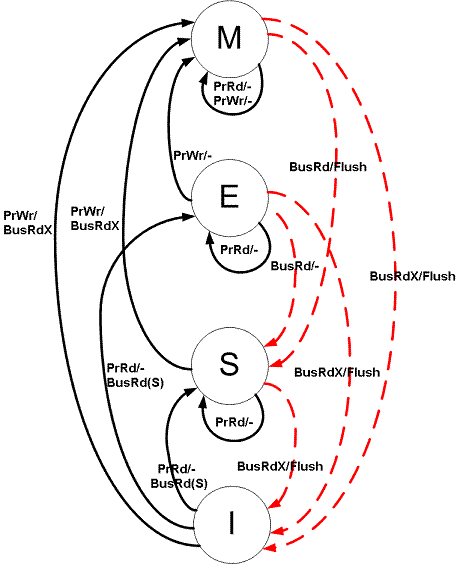
\includegraphics[scale=0.4]{img/mesi.png}
  \caption{Protocol MESI}
  \label{fig:Protocol MESI}
\end{figure}

% 3.2
\section{Memory consistency}
In a multiprocessor environment such as the IBM Power System AC922 Power9, the memory consistency is essential to
ensure that all cores share a coherent view of the data stored in memory. The Power9 implements memory consistency
models, such as the Total Store Order (TSO) model, which establishes rules for how read and write operations should
be coordinated between cores. This ensures that, when accessing and modifying shared data, all cores see a consistent
version of the information. In other words, memory consistency in Power9 takes care of maintaining the integrity of
data shared between multiple cores, avoiding potential conflicts and ensuring predictable behaviour.

% Nueva página
\cleardoublepage

% 3.3
\section{Thread and processor synchronisation}
Synchronisation refers to the efficient coordination of activities between threads and processors. In Power9, this
process is handled by specific instructions such as \emph{sync} and \emph{lwsync}. These instructions act as
synchronisation points, ensuring that memory operations are performed in the proper order and avoiding problems such
as race conditions, where multiple threads attempt to access or modify the same memory location simultaneously.
Synchronisation in Power9 ensures that memory operations are executed in an orderly and coherent manner across 
different elements of the system, contributing to efficient and predictable performance in multiprocessor environments.

% Capitulo 4
\chapter{Interconnection networks}
\section{Switching techniques}
The main interconnection networks that the IBM Power System AC922 has are the following:

\setlength{\parindent}{1em}
\CIRCLE \ \ \textbf{NVLink 2.0:} It is a high-speed interconnect technology that enables exceptional communication between 
the processor and accelerator. NVLink 2.0 is the second generation of this technology, delivering up to 25 GBps per 
link, which means each GPU can have up to 150 GBps bandwidth to the processor and up to 300 GBps bandwidth to other
GPUs. The IBM Power System AC922 has up to six dedicated NVIDIA Tesla V100 GPUs, which connect to the POWER9 processor
via NVLink 2.0. This enables high performance and low latency in parallel computing-intensive applications such as 
artificial intelligence, machine learning or scientific simulation.

\noindent Some features are:

\setlength{\parindent}{2em}
- It has a coherent architecture, which allows the processor and GPUs to share the same physical and virtual memory, reducing the overhead of copying data between devices.

- It has an error-correcting technology, which ensures data integrity and system reliability.
\setlength{\parindent}{0em}


\begin{figure}[H]
  \centering
  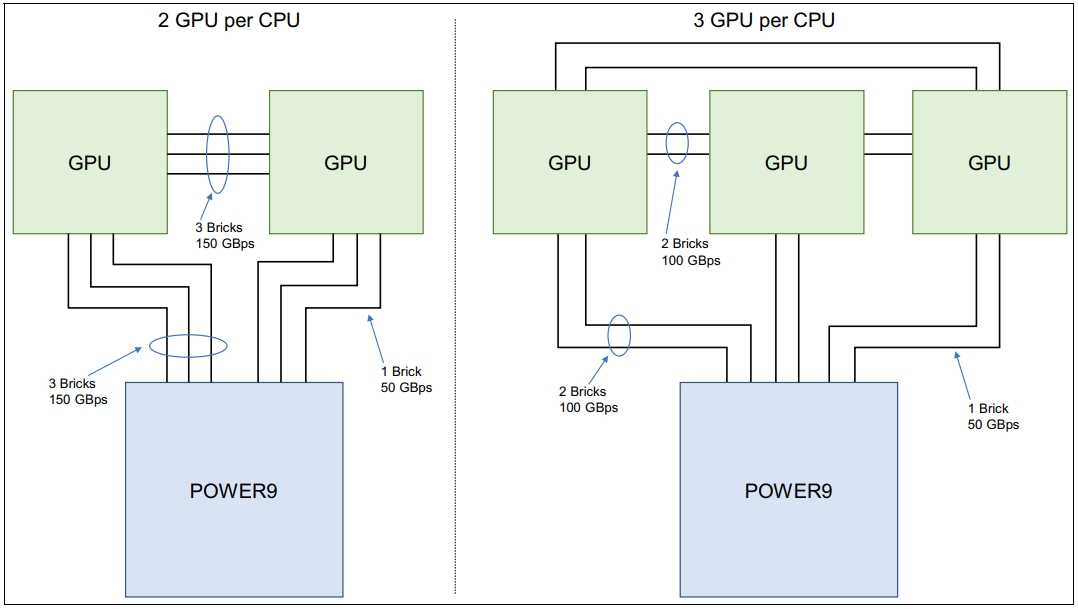
\includegraphics[scale=0.52]{img/NVLink.jpg}
  \caption{General scheme of NVLink 2.0}
  \label{fig:General scheme of NVLink 2.0}
\end{figure}

% Nueva página
\cleardoublepage

\setlength{\parindent}{1em}
\CIRCLE \ \ \textbf{OpenCAPI:} The Power System AC922's OpenCAPI network is one of the most advanced interconnect 
networks available. OpenCAPI is an open standard that allows high-performance devices, such as solid-state drives 
(SSDs) or accelerator cards, to be connected directly to the Power9 processor, bypassing the PCI Express bus.
This enables faster and more efficient communication with very low latency and very high bandwidth.

\setlength{\parindent}{0em}
The Power System AC922's OpenCAPI network has four slots on the motherboard, which support OpenCAPI 3.0 devices.
Each slot offers a data transfer rate of up to 25 GB/s, more than doubling the speed of PCIe Gen4 slots, which
offer up to 16 GB/s. In addition, the OpenCAPI network enables coherent access to processor memory, making 
OpenCAPI devices easier to program and use.

\begin{figure}[H]
  \centering
  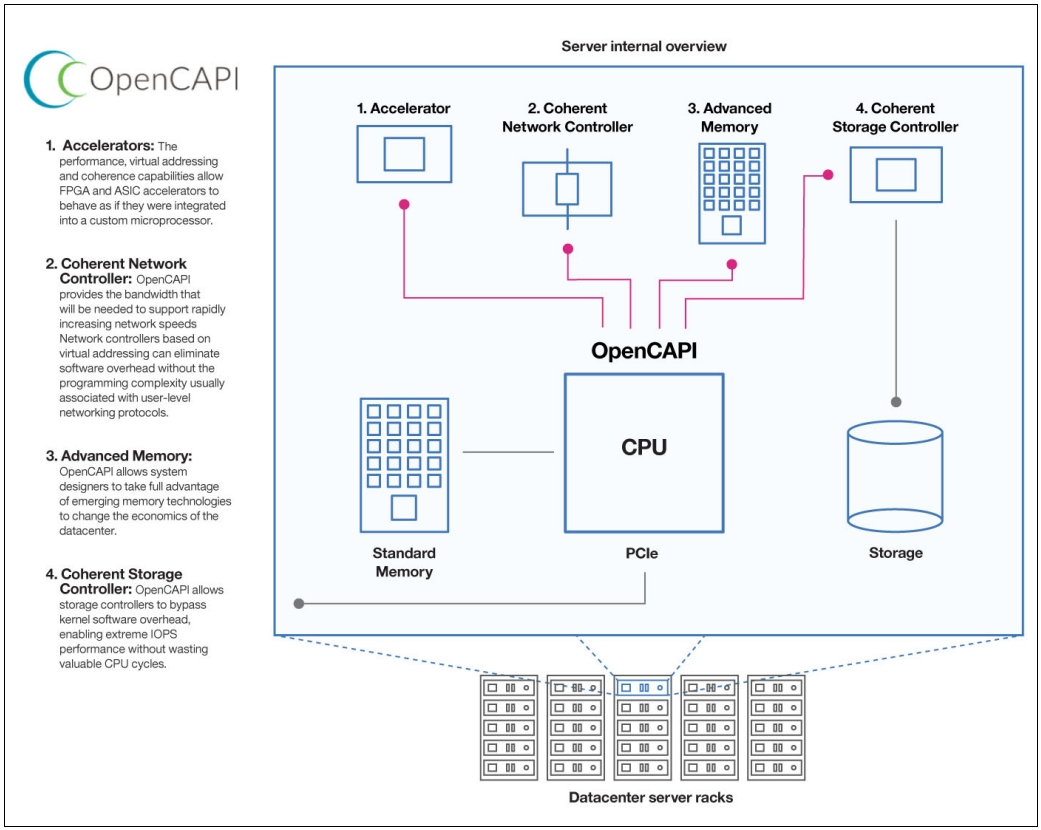
\includegraphics[scale=0.5]{img/opencapi.jpg}
  \caption{General scheme of OpenCAPI}
  \label{fig:General scheme of OpenCAPI}
\end{figure}

\setlength{\parindent}{1em}
\CIRCLE \ \ \textbf{PCIe Gen4:} It is the fourth generation interconnect standard for peripheral devices such as
network cards, disk controllers or sound cards. PCIe Gen4 offers a data transfer rate of up to 16 GB/s per link.
The IBM Power System AC922 has multiple PCIe Gen4 slots that allow you to connect high-speed devices and expand 
the capabilities of the system. This allows for greater scalability and compatibility with existing devices.

% Nueva página
\cleardoublepage

\noindent The following image shows a general diagram of the interconnection networks of the IBM Power System AC922:

\begin{figure}[H]
  \centering
  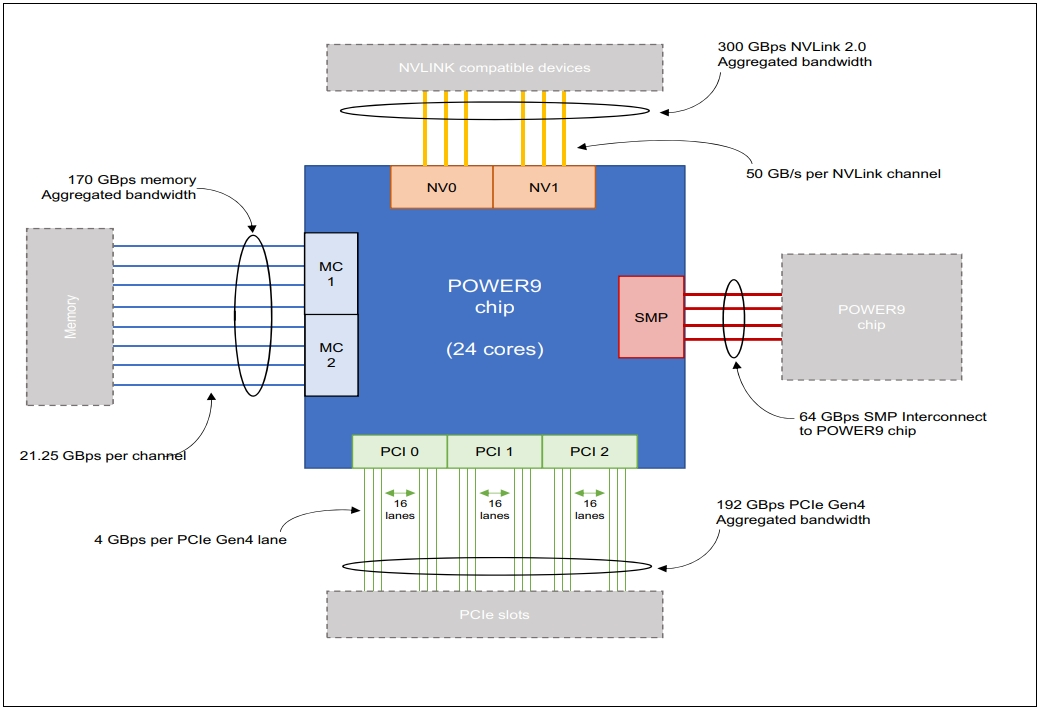
\includegraphics[scale=0.5]{img/esquema_general.jpg}
  \caption{General schematic of the IBM Power System AC922 interconnection network}
  \label{fig:General schematic of the IBM Power System AC922 interconnection network}
\end{figure}

\section{Network topologies}
\noindent The IBM Power System AC922 has several network topologies, which allow the different components of the system
to be connected in an efficient and scalable way. The topologies are as follows:

\CIRCLE \ \ \textbf{Fat tree topology:} They are regular and indirect topologies based on complete trees.

\CIRCLE \ \ \textbf{Mesh or All-to-all topology:} Although usually described as a direct topology, meshes can also be 
indirect. In the first case, each node connects directly to the others. In the second case, each node is connected to 
the network via a link and a switch.

\CIRCLE \ \ \textbf{2D-tours topology:} It is a direct topology based on a two-dimensional mesh. The nodes are connected to each other

\CIRCLE \ \ \textbf{3D-tours topology:} It is a direct topology based on a three-dimensional mesh. The nodes are connected to each other

\CIRCLE \ \ \textbf{5D-tours topology:} It is a direct topology based on a five-dimensional mesh. Nodes are connected to each other

\CIRCLE \ \ \textbf{Dragonfly topology:} It is based on the idea of a ``swarm'' of connections between groups of compute nodes. Instead 
of having a single global network, Dragonfly connects multiple clusters of nodes called ``islands'' or ``pods''.

\CIRCLE \ \ \textbf{Hypercube topology:} It is the connection of nodes in a multidimensional space in such a way that each node is directly
connected to other nodes that differ by a single bit. directly to other nodes that differ by a single bit.

% Nueva página
\cleardoublepage

\chapter{Conclusion}
\noindent The IBM Power System AC922 has become a leading choice for organisations seeking advanced and efficient computing power, 
especially those working in fields such as artificial intelligence, deep learning and high-performance scientific research. Its 
robust design and ability to handle demanding workloads position it as a leading choice in the high-performance computing landscape.

\chapter{Bibliography}
\setlength{\parindent}{0em}
Nohria, R., Santos, G., \& Haug, V. (2018). \emph{IBM Power System AC922 Technical Overview and Introduction}. \url{https://www.redbooks.ibm.com/redpapers/pdfs/redp5494.pdf}

top500. (2022) \emph{SUMMIT - IBM POWER SYSTEM AC922, IBM POWER9 22C 3.07GHZ, NVIDIA VOLTA GV100, DUAL-RAIL MELLANOX EDR INFINIBAND}. \url{https://top500.org/system/179397/}

IBM. (2021). \emph{8335-GTX (IBM Power System AC922)}. \\ \url{https://www.ibm.com/docs/es/power9?topic=8335-gtx-power-system-ac922}

Wikipedia. (2023). \emph{Power9}. \url{https://en.wikipedia.org/wiki/POWER9}

\end{document}